% !TEX root = migratedoc.tex
\chapter{A quick overview of the calculations and specification of the parameters}
\myabstract{A short overview of the math that is used by the program \migrate. If you want to treat \migrate as a black box, then skip to the section on \textbf{parameter definitions}.}
The program \migrate infers population genetic parameters from genetic data. Essentially we want to find the  Bayesian posterior probability density of parameters $\P$ of a particular model given the Data $\Dd$:
\begin{align}
   \prob(\P | \Dd). \notag
\end{align} 

This posterior probability density of the population genetics parameters $\P$, 
such as population sizes or migration rates, can be calculated in principle by integrating over all possible 
relationships 
$\G$ 
of the sample data 
$\Dd$ 
using   an expansion of the coalescent theory \citep{kingman1982-27,kingman1982-235,kingman2000-1461} which
includes migration \citep{hudson1991-1,nath1993-841,notohara1990-59} and/or population splitting \citep[for example, ][]{nielsen:1998:mle}.
\begin{align}
\prob(\P | \Dd) &=  \frac{\prob( \P, \Dd)}{\prob(\Dd)} \\
\intertext{which is equivalent to Bayes formula:}
\prob(\P | \Dd) &=  \frac{\prob(\P) \prob( \Dd | \P)}{\prob(\Dd)}.\\
\intertext{The famous Bayes formula is very general and discusses little what needs to be done in detail, but we want to estimate the probability of particular model parameter values for a given dataset. This posterior probability density depends on the likelihood of the data given the parameters and its priors scaled by the integral over all parameters. the denominator is a simple scaler to make the left hand side a proper probability. the likelihood is problematic because for our problem we need to relate the data (genetic material) with a model about populations. We can achieve that by using random genealogies and weight them how  well they fit the data. We simple could consider all genealogies of our sampled data and integrate over them and use}
\label{BAYES}
\prob(\P | \Dd) &=  \frac{\prob(\P) \int_G \prob(G | \P) \prob( \Dd | G)dG}{\prob(\Dd)}.  \\ 
\intertext{The likelihood calculations is the most problematic because of the integration over genealogies}
\label{LIKELIHOOD}  
{\mathrm L}(\P) = \prob(\Dd | \P) &=   \int_G \prob(G | \P) \prob( \Dd | G)dG.   
\end{align}
 The key issue is that there are huge number if different topologies, each with continuous branch lengths; it  is a sum over all possible labeled histories and integrals over all possible branch lengths $b_i$
\begin{align}
{\mathrm L}(\P) &= \sum_T \int_{b_1} ... \int_{b_k} \prob(T,\underline{b} | \Theta) \prob(\Dd | T,\underline{b}) db_1...db_k.
\end{align}
Older versions of \migrate than version 4.0 could use both approaches to estimate the parameters. It became a major burden updating the program to maintain both likelihood and Bayesian inference, so that I decided to strip out the likelihood material and focus on the Bayesian approach, which is often easier to code and maintain. One of the major headaches with the likelihood approach was the maximization of the likelihood function that became more and more complicated with more parameters, this maximization is not needed in the Bayesian approach, although we still need to calculate likelihoods.

\subsection{\textcolor{red}{Parameter specification and definition}} 
\migrate needs a population model and this model is framed in parameters that describe population sizes and geneflow between populations.
Specifically, \migrate estimates migration rates, population splitting times, and effective population sizes of 1 to many populations
using genetic data (Fig 1).  The parameters to estimate are
\begin{align}
\label{PARAMETERS}
\P &= \left(\begin{matrix}  \underline{\Theta} & \underline{\M} & \underline{\Delta} & \underline{S_\Delta}\end{matrix}\right),
\end{align}
where $ \underline{\Theta}$ are the mutation-scaled population sizes of each subpopulation, using $\Theta=xN_e\mu$, where $x$ is the inheritance scalar, which is for diploids 4 and for haploids 2; $N_e$ is the effective population size ; and $\mu$ is the mutation rate per site and per generation with DNA/RNA data, for microsatellite data $\mu$ is for the whole locus per generation. $ \underline{\M}$ are the mutation-scaled immigration rates which are $m_{i\rightarrow j} / \mu$, $m_{i\rightarrow j}$ is the rate of immigration into population $j$ from $i$ per generation. The direction is interpreted in a standard population genetics way: an individual is in population $i$ at time $z$ and then either its gametes or itself arrives in population $j$ at time $z+1$. The theory does not really consider the emigrants (similarly we do not worry about the many gametes that we do not choose between generations, only the ones that make into the next generation or, here, into the other population or stay are relevant. The divergence parameters $\Delta_{i\rightarrow j}$ and $S_{\Delta, i\rightarrow j}$ are the parameters of a distribution (commonly a normal) that express the divergence time and its standard deviation. The divergence time is the time where a descendent $j$ splits off of the ancestor $i$, the ancestor $i$ can but need not to be a sampled population. The divergence time is similarly scaled as the other parameters and \migrate estimates a mutation-scaled divergence time. The time is measured in generation times the mutation rate per site and generation. For comparison to other software you may want to divide the divergence time by the sum of all scaled population sizes to scale the time in coalescent units. This works well when compared to the simulation software \ms \citep{hudson2002}.
  
\section*{Mutation-scaled population sizes}
\vskip -1cm 
\begin{align}
\underline{\Theta} &= \left( \begin{matrix} \Theta_1 & \Theta_2 & ... & \Theta_n \end{matrix} \right)
\end{align}
where each $\Theta_i = x N_e \mu$ with $\mu$ that is the mutation rate per generation and with $x$ that is a multiplier that depends on the ploidy and inheritance of the data, for nuclear data it $x=4$, for haploid data it is $x=2$, and for mtDNA in vertebrates with female-only transmission, no sex-change during its life, and a sex ratio of 1:1, it is $x=1$. Life history is important, for example some fish species, such as Grouper, change sex in their lifetime and therefore all individuals can transmit mtDNA resulting in having $x\simeq2$ and not $x=1$. 

\section*{Mutation-scaled immigration rates}
\vskip -1cm 
\begin{align}
\underline{\M} &= \left( \begin{matrix} - & \M_{2 \rightarrow 1} & \M_{3 \rightarrow 1} & ... & \M_{n \rightarrow 1} \\  \M_{1 \rightarrow 2} & - & \M_{3 \rightarrow 2} & ... & \M_{n \rightarrow 2}\\ 
... & ... & ... & ... & ... \\
\M_{1 \rightarrow n}  & ... & ... & \M_{(n-1) \rightarrow n}  & - \end{matrix} \right)
\end{align}

which is the immigration rate per generation $m$ divided by the mutation rate per generation $\mu$, it is a measure of how much more important immigration is over mutation to bring new variants into the population. The traditional number of immigrants per generation $xN_im_{j\rightarrow i}$ is  $\Theta_i\M_{j\rightarrow i} = xN_{i}\mu \times m_{j\rightarrow i} / \mu = xN_im_{j\rightarrow i}$. The mutation rate $\mu$ is per site and generation for DNA data and per locus and generation for microsatellite or allelic data. If you compare results of different programs make sure that you understand what are the units of $\mu$, oftentimes it $\mu$ per locus even with DNA data!

There seems to be considerable confusion about migration directions in the recent literature. When Sewall Wright discussed migration, he considered immigration rate into a population, and since we do not observe immigrants directly, he also assumed that our data represents the offspring of locals and immigrants. In his framework he did not consider emigration and  that immigration will happen instantaneous (e.g no delayed influx of gene through seed banks etc). If we see $\M_{2 \rightarrow 1}$ then we always use a forward time perspective: in the past the individual was in population 2 and now is in population 1. 

The immigration parameter in \migrate is a longtime average over the genealogy of the individuals in the sample. This works well for populations that fluctuate around a value, but even with mildly growing populations this works fine, only with strongly growing populations one may get underestimates using \migrate.   
\begin{figure}[htb]
\begin{center}
\leavevmode
\hbox{%
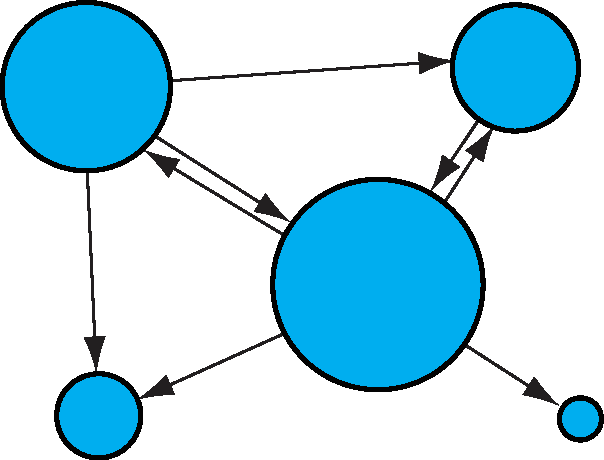
\includegraphics[scale=0.6]{mim/example-migration-lightblue}}
\end{center}
\begin{picture}(0,0)(0,0)
\put(76,50){$M_{14}$}%
\put(75,40){$M_{12}$}%
\put(52,26){$M_{13}$}%
\put(103,20){$M_{15}$}%
\put(89,42){$M_{42}$}%
\put(70,22){$M_{23}$}%
\put(67,32){$M_{21}$}%
\put(102,36){$M_{24}$}%
%
\put(59,45){$\Theta_1$}
\put(89,25){$\Theta_2$}
\put(52,14){$\Theta_3$}
\put(103,48){$\Theta_4$}
\put(115,13){$\Theta_5$}
\end{picture}

\caption{Populations exchanging migrants with rate $m_{j \rightarrow i}$ per generations and with size 
$N_e$. The parameters are scaled by mutation rate $\mu$ which is with sequence data per site per generation. The estimated parameters are therefore: $\Theta_i$ which is $x N^{(i)}_e \mu$ and 
$\M_i$ 
which is $m_i/\mu$, the migration estimate is often also expressed as $xNm$ which is just $\Theta \M$, x is the inheritance parameter and depends on the data, commonly 4 for nuclear data, and 1 for mtDNA data. The example model is not a complete (full) model because some migration routes are not estimated and set to zero.}
\label{FIG1}
\end{figure}



\begin{figure}[tbh]
\begin{center}
\leavevmode
\hbox{%
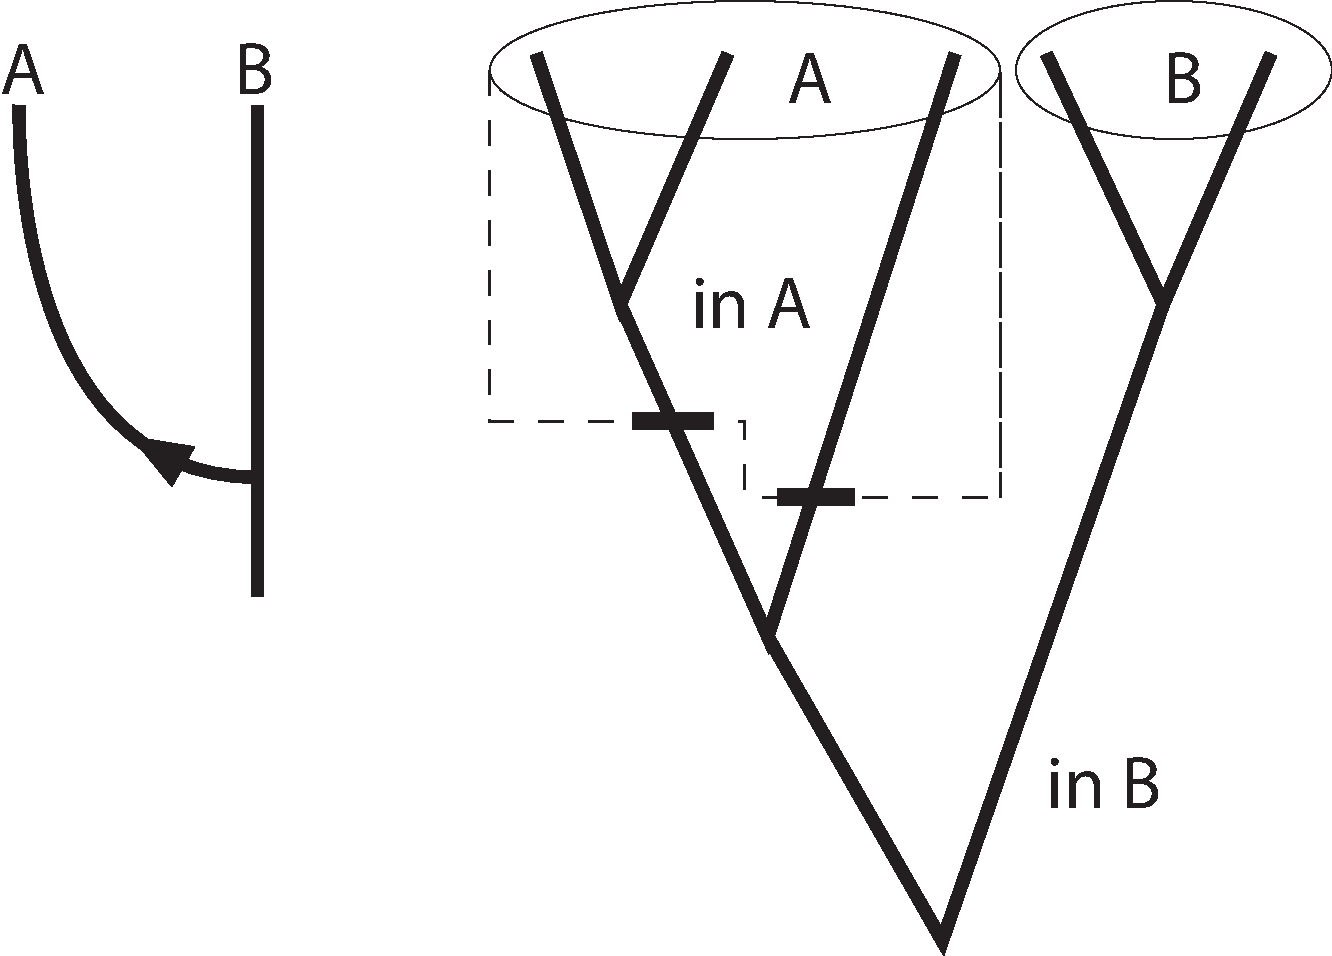
\includegraphics[scale=0.4]{mim/species_manual}}
\end{center}

\caption{Populations splitting, left is the model specification, two populations A and B, A splits off B. Right, detail view for the gene tree. Each individual can split off by itself.}
\label{FIG2}
\end{figure}

\section*{Mutation-scaled population splitting  times $\Delta$ and standard deviations $S_\Delta$}
The population splitting times are model differently to other programs that all use the model of IM \citep{Hey:2010a}.
Our new model was described by \cite{beerli2019b}.  We treat population splitting events as individual events on a lineage. Looking backward in time, a lineage $\ell$  currently in population $\kappa$ is at risk of being  in a different population either by migration with rate $\M$ or into another population by a splitting event. The Splitting event is proposed during the MCMC run using a hazard function of the splitting time distribution, for simplicity we use a truncated Normal distribution with mean $\Delta$ and standard deviation $S_\Delta$. Drawing these splitting events using a hazard function is equivalent to the coalescent or migration event which are also hazard functions. During the MCMC runs many different splitting events will be proposed from the Normal distribution with $\Delta_j$ and $S_{\Delta_j}$ for $j$ population splits. The current version needs guidance which populations are merging (looking backwards in time), for an example see the Bayes Factor section.  In the parmfile and the menu the setting of the splitting parameters is combined with setting the migration model, for an example see definition of the custom migration matrix.  


%\section{Maximum likelihood estimation of migration rates}
%The estimates of the parameters $\P$ are found by maximizing formula (\ref{LIKELIHOOD}.)
%We bias the search path through all trees towards trees with higher likelihoods (Fig. 2)
%and have then to correct for this. The likelihood formula changes to
%\begin{align}
%\frac{L(\P)}{L(\P_0)} &= \frac{1}{m}\sum_i^m\ \frac{ \prob(D\ |\ g_i)\ \prob( g_i\ |\ \P)}
%{\prob(D\ |\ g_i)\ \prob( g_i\ |\ \P_0)}.
%\end{align}
%Such an approach is reasonable because summands with low probabilities
%will contribute very little to the final likelihood. For more information on the base model, you should read \cite{beerli:1999:mle} and \cite{kuhner1995-1421}.
%
%The approximation of the likelihood using a ratio makes it difficult to
%compare different runs of the program. The program reports a likelihood
%that is actually a ratio of likelihoods and since we recalculate the
%parameters for each chain, the values for $\P_0$ are different
%between runs, and therefore it is impossible to compare them. A comparison of the parameters, of course, is still possible.
%An escape of this 
%problem is to run the program using the full model (e.g. $n \times n$ parameters and use the likelihood ratio test for specific scenarios.
%
\section{Bayesian inference}
\migrate estimates the parameters using a Bayesian paradigm (see formula \ref{BAYES}), simulation studies of simple models show that there are few differences with the ML runs, although some combinations of parameters might be be easier to estimate with the Bayesian approach \citep{beerli:2006:CBM}. One of the bigger problems with the Likelihood approach is the effort that has to be made to calculate the confidence intervals of the best estimates, default analyses often led to narrow support intervals thus making researchers overconfident about the explanatory power of their data; the use of the prior distribution seems to make a Bayesian approach less vulnerable to this problem. Bayesian inference is commonly based on Markov chain Monte Carlo (MCMC) because we usually cannot integrate the function of interest analytically or by simple numerical approach. MCMC was described first by \cite{Metropolis:1953:ESC} and refined by \cite{hastings1970-97}. For an introduction see \cite{Hammersley:1964:MCM}or \cite{chib:1995:umh}, 
and see \cite{kuhner1995-1421} for a first application using MCMC in the context of coalescence theory.

\begin{figure}[tbh]
\begin{center}
\leavevmode
\hbox{%

\includegraphics[scale=0.8]{mim/planes_orig}}
\end{center}
\caption{
(A) On an imaginary, infinite likelihood surface  we would need to sample every possible
genealogy and sum all these values which is not possible, but trees with low probability will not contribute much to the final likelihood,  (B) by biasing towards better trees we can sample effectively from those trees with high 
contribution to the final likelihood and can approximate the likelihood (\ref{LIKELIHOOD}).
}
\label{FIG3}
\end{figure}

%In principle, we do not need to integrate at all with MCMC but sample parameter values during the run and build a histogram for the parameters of interest.
Commonly we think of the marginal posterior distribution of each parameter (summing/integrating over all 'nuisance' parameters). We use particular values to drive the MCMC, and in a Bayesian analysis we get them from the Prior distribution, this may help to get good results in situations where the data suggests a very rough landscape of parameter- and tree-space (see Fig. \ref{FIG3} for an example with a smooth surface). \migrate allows using several different prior distributions, some are more appropriate for you data than others. I often suggest to use the uniform prior distribution because it is simple and shows obvious deficiencies in an analysis very quickly, but it also tends to increase the credibility intervals because it supports very large or very small parameter values equally. This may sound as an odd choice because for example we know that the population size of humans never was zero and never was $10^{10}$, so a uniform prior distribution with range 0 to $10^{10}$ does not sound right although such a prior would do fine in an analysis because the data is strong enough to suggest that the posterior probability near a size of zero is close to zero and the probability of a size of $10^{10}$ is also small.
 
%The parameter $r$ is the a uniform random number from (0,1].

\subsection{Prior distributions}
\vskip -0.5cm
\subsubsection{Uniform prior distribution}
The parameters have a uniform distribution between a minimal and a maximal value of the parameters, there is a set of minima and maxima for $\underline{\Theta}$ and $\underline{\M}$.
\migrate calculates the uniform by using
\begin{gather}
\label{UNIPRIOR}
    \prob(\P_i) =  \frac{1}{\P_{max} - \P_{min}} \\
    \intertext{it is implemented using a windowing method with window size $\Delta$, that is preferrably around 1/10 of the whole range.}
    \P_{\mathrm new} =  \P_{\mathrm old} + (2 \Delta r - 1) \begin{cases} \P_{\mathrm new} < \P_{\mathrm min}  &  \P_{\mathrm min} + |\P_{\mathrm min} - \P_{\mathrm new}| \\
     \P_{\mathrm new} > \P_{\mathrm max}  &  \P_{\mathrm max} - |\P_{\mathrm max} - \P_{\mathrm new}| \end{cases}
\end{gather}

\subsubsection{Gamma distribution prior}
The truncated gamma distribution has four parameters $\alpha$, $\beta$, minimum $a$, and maximum $b$. The gamma prior in \migrate is defined through the mean $\mu$, $\alpha$, $a$, and $b$ 
\begin{gather}
\label{GAMMAPRIOR}
% (E^(-(x/\[Beta])) x^(-1 + \[Alpha]) \[Beta]^-\[Alpha])/Gamma[\[Alpha]] mathematica standard Gamma
%
\alpha = \mu / \beta\\
\beta = \text{minimization of the mean of the truncated gamma and the parameter $\mu$}  \\
\prob(\P_i) =  \text{probability of the truncated gamma} 
%    \intertext{it is implemented using a windowing method with window size $\Delta$, that is preferrably around 1/10 of the whole range.}
%    \P_{\mathrm new} =  \P_{\mathrm old} + (2 \Delta r - 1) \begin{cases} \P_{\mathrm new} < \P_{\mathrm min}  &  \P_{\mathrm min} + |\P_{\mathrm min} - \P_{\mathrm new}| \\
%     \P_{\mathrm new} > \P_{\mathrm max}  &  \P_{\mathrm max} - |\P_{\mathrm max} - \P_{\mathrm new}| \end{cases}
\end{gather}



\subsubsection{Exponential prior distribution}
The parameters have a exponential distribution, \migrate calculates three versions\\
\textsl{Simple exponential prior distribution}
\begin{align}
\label{EXPPRIOR}
    \prob(\P_i) &=  \int_0^\infty exp( -P_{i} / P_{\mathrm mean}) / P_{\mathrm mean} d\P_i = exp(- P_{i}/P_{\mathrm mean}) \\
    \P_{\mathrm new} &=  - \P_{\mathrm mean}\ ln(r)
\end{align}
\textsl{Exponential prior distribution with fixed window}
\begin{align}
\label{WEXPPRIOR}
    \prob(\P_i, \P_{\mathrm min}, \P_{\mathrm max}) &=  \frac{\int_{\P_{\mathrm min}}^{\P_{\mathrm max}} exp( -P_{i} / P_{\mathrm mean}) / P_{\mathrm mean} d\P_i}{exp(-P_{\mathrm min}/P_{\mathrm mean}) - exp(-P_{\mathrm max}/P_{\mathrm mean})}\\ 
     &= \frac{exp(-P_{\mathrm min}/P_{\mathrm mean}) - exp(-P_{\mathrm x}/P_{\mathrm mean})}{exp(-P_{\mathrm min}/P_{\mathrm mean}) - exp(-P_{\mathrm max}/P_{\mathrm mean})} \\
    \P_{\mathrm new} &=  - \P_{\mathrm mean}\ ln(\frac{r}{exp(\P_{\mathrm max}/\P_{\mathrm mean})}-\frac{r-1}{exp(\P_{\mathrm min}/\P_{\mathrm mean})}); 
\end{align}
\textsl{Exponential prior distribution with variable window}
\begin{align}
\label{AEXPPRIOR}
    \prob(\P_i | \P'_i,  \P_{\mathrm min}, \P_{\mathrm max}) &=  \frac{2 \int_{\P'_i - \Delta}^{\P'_i + \Delta} exp( -P_{i} / P'_i) / P'_i d\P_i}{exp(1) Csch(\Delta / P'_i)}\\ 
     &= \frac{(exp(\Delta + P_i)/P'_i - exp(1)) Csch(\Delta/\P'_i)}{2 exp(\P_i/\P'_i)} 
     \end{align}
     \begin{align}
    \P_{\mathrm new} &=  \P'_i - \P'_i ln(exp(\Delta/\P'_i) - 2 r Sinh(\Delta / \P'_i))\begin{cases} \P_{\mathrm new} < \P_{\mathrm min}  &  \P_{\mathrm min} + |\P_{\mathrm min} - \P_{\mathrm new}| \\
     \P_{\mathrm new} > \P_{\mathrm max}  &  \P_{\mathrm max} - |\P_{\mathrm max} - \P_{\mathrm new}| \end{cases}
\end{align}
